\documentclass[aspectratio=169]{beamer}
\usetheme{Madrid}
\usepackage[utf8]{inputenc}
\usepackage[T1]{fontenc}
\usepackage{tikz}
\usepackage{amssymb}
\usepackage{graphicx}
\setbeamertemplate{navigation symbols}{}
\setbeamercolor{title}{fg=white,bg=blue!70!cyan}
\setbeamercolor{frametitle}{fg=white,bg=blue!70!cyan}
\setbeamercolor{block title}{bg=blue!70!cyan!20,fg=black}
\setbeamercolor{block body}{bg=blue!70!cyan!8,fg=black}
\setbeamercolor{item}{fg=blue!70!cyan}
\setbeamercolor{itemize item}{fg=blue!70!cyan}
\setbeamertemplate{itemize item}[triangle]

\title{G2 — Variables \& State}
\subtitle{Score, health, timers — numbers that change}
\author{ByteForge --- Grade 7 --- Game Maker}
\date{}

\begin{document}

\begin{frame}
    \titlepage
\end{frame}

\begin{frame}{Today's Plan}
    \begin{itemize}
        \item Colour Square
        \item Growing Circle
        \item Health Bar
        \item[$\bigstar$] BOSS --- Clicker Upgrade
    \end{itemize}
\end{frame}

\begin{frame}{Variables — a named box that can change}
    \large
    \begin{itemize}
        \item R, g, b hold numbers 0-255 for red/green/blue
        \item Using a variable READS its value; only a "set"/"change" block updates it.
    \end{itemize}
\end{frame}


\begin{frame}{One variable, many uses}
    \large
    \begin{itemize}
        \item Change size once, and every place that reads it shows the new value
        \item That's the whole point of variables.
    \end{itemize}
\end{frame}


\begin{frame}{A variable driving TWO different things}
    \large
    \begin{itemize}
        \item Health drives a bar's WIDTH directly
        \item The "one variable, automatically reflected in visuals" pattern behind every health/progress bar.
        \item Worked example: health at 100 draws a full-width bar; health at 20 draws a bar only one-fifth as wide — the SAME width calculation (health / max * barWidth) every single frame, no special "low health" case needed.
    \end{itemize}

    \begin{center}
    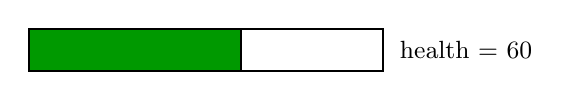
\begin{tikzpicture}[scale=0.9]

        \draw[thick] (0,0) rectangle (5,-0.6);
        \draw[thick, fill=green!60!black] (0,0) rectangle (3,-0.6);
        \node[right] at (5.1,-0.3) {\small health = 60};
    \end{tikzpicture}
    \end{center}
\end{frame}


\begin{frame}{BOSS — a variable that changes over time}
    \large
    \begin{itemize}
        \item A variable, a frame loop, and an IF working together
        \item Score only rises when Space is held.
    \end{itemize}
\end{frame}

\begin{frame}{Real-World Examples}
    \large
    \begin{itemize}
        \item Any RPG or shooter's health bar visibly shrinking as you take damage
        \item The bar's pixel width is driven directly by one number, exactly like this chapter's health-bar challenge. Minecraft's ten hearts are the same idea drawn as icons instead of a bar
        \item Hearts remove as the health variable drops.
    \end{itemize}
\end{frame}


\begin{frame}{Let Them Discover}
    \Large
    Find a game with a visible health or loading bar. Watch it shrink or fill — does it move in smooth small steps, or big jumps? What does that tell you about how often the variable is being redrawn?
\end{frame}

\begin{frame}{Your Turn}
    \Large
    Open the student map, find \textbf{G2 — Variables \& State}, and work through it
    hands-on --- everything you just saw, they now do themselves.
\end{frame}

\end{document}
